\chapter{Methodik und Ergebnisse}

\section{Patentdatensatz}
Der Patentdatensatz enthält ausschließlich Patente von \acl{gm} (\ac{gm}), die durch das Tochterunternehmen \ac{gm} Global Technology Operations angemeldet wurden. Mit der Suchanfrage ((AN/\enquote{GM Global} AND ((ICL/F16H\$ AND APD/20040101->20121231) OR (CPC/F16H\$ AND APD/20130101->20181231))) AND ISD/20040101->20181231) \todo[inline]{diese Gänsefüßchen muss man in der Suchanfrage bis jetzt manuell ersetzen} lassen sich die 1411 Dokumente auf der Internetseite des United States Patent and Trademark Office einsehen. 
%http://patft.uspto.gov/netacgi/nph-Parser?Sect1=PTO2&Sect2=HITOFF&p=1&u=%2Fnetahtml%2FPTO%2Fsearch-adv.htm&r=0&f=S&l=50&d=PTXT&Query=AN%2F%28%22GM+Global%22%29+AND+%28%28ICL%2FF16H%24+AND+APD%2F20040101-%3E20121231%29+OR+%28CPC%2FF16H%24+AND+APD%2F20130101-%3E20181231%29%29+AND+ISD%2F20040101-%3E20181231

\section{Preprocessing}
Das Preprocessing wurde mit dem PatVisor\textregistered, das Patentanalysewerkzeug vom \acl{ipmi} (\ac{ipmi}), durchgeführt. Dazu wurde vom \ac{ipmi} ein themenbezogener Synonymfilter bereitgestellt. Aus den Patenten wurde nur der Titel, der Abstract und die Claims als Text verwendet. Die Anmeldedaten wurden als Metadaten für \ac{dlda} verwendet. Die Texte wurden mit dem Patvisor lemmatisiert. Das Lemma ist die Grundform eines Wortes und wird hier verwendet damit die Häufigkeit des Wortes bestimmt werden kann, einschließlich aller Varianten. Herausgefiltert wurden Artikel, Pronomen und Ähnliches das nur im Kontext eine Bedeutung hat und daher im \acl{bow} Modell irrelevant ist. Außerdem wurden manuell Abkürzungen erfasst wie \acl{cvt} (\ac{cvt}). Bigramme wurden in einem Fenster von fünf Worten erstellt, das über den Text rolliert. Die Worte eines Fensters wurden ohne Wiederholung permutiert. Die Wörter in einer \acl{tdm} (\ac{tdm}) gespeichert.

\section{Durchführung des Topic Modeling}

\subsection{LDA}
Das Topic Modeling wurde nach dem Preprocessing in vier Schritten implementiert: Wörterbuch- und Korpuserzeugung, \ac{lda}, Evaluation, Visualisierung. Gensim ist eine Python library für Textanalyse. Ein Teil des Codes wurde vom IPMI bereitgestellt. Zuerst wird aus der \ac{tdm} des Preprocessings ein Wörterbuch und ein Korpus erstellt. Das Wörterbuch indiziert jedes Wort und speichert die Häufigkeit des Wortes aus dem gesamten Korpus. Der Korpus verbindet die Indizes der Wörter mit den Indizes der Dokumente und speichert die Häufigkeit der Wörter pro Dokument.

\begin{table}[!htb]
	\RawFloats
	\begin{minipage}{.5\linewidth}
		\caption{Wörterbuch}
		\centering
		\begin{tabular}{|c|c|c|}
			\hline 
			Dokument ID & Wort ID & Häufigkeit \\ 
			\hline 
			1& 5 &65  \\ 
			\hline 
			1& 10 & 20 \\ 
			\hline 
			2& 11 & 11 \\ 
			\hline 
		\end{tabular} 
	\end{minipage}%
	\begin{minipage}{.5\linewidth}
		\centering
		\caption{Korpus}
		\begin{tabular}{|c|c|c|}
			\hline 
			Wort ID & Wort & Häufigkeit \\ 
			\hline 
			1923& ability & 3 \\ 
			\hline 
			2049& aboard &3  \\ 
			\hline 
			1404& abort & 5 \\ 
			\hline 
		\end{tabular} 
	\end{minipage} 
\end{table}

Ein Thema wird für Menschen durch die wahrscheinlichsten Wörter ersichtlich. \parencite[vgl.][S. 265-266]{mimno2011optimizing} Mit der Kohärenz eines Themas ist der semantische Zusammenhang zwischen diesen Wörtern gemeint. Diese Kohärenz kann man durch das gemeinsame Auftreten von Wörtern in einer Gruppe berechnen. Das u\_mass Maß funktioniert nach diesem Prinzip, benannt nach der Universität von Massachusetts. Es gibt auch andere Kohärenzmaße wie das c\_v Maß, die eine bestimmte Anzahl an Wörtern in einem Schiebefenster betrachten. Dadurch wird ein feinerer Kontext betrachtet anstatt das gesamte Dokument. Allerdings wird hier u\_mass verwendet, weil es aufgrund des fehlenden Schiebefensters auch bei Bigrammen funktioniert.

Die Distanz zwischen zwei Themen ist die Unterschiedlichkeit der Wörter zweier Themen. Eine Methode der Berechnung ist der Jaccard-Koeffizient. Diese ist die Mächtigkeit der Schnittmenge dividiert durch die Mächtigkeit der Vereinigungsmenge zweier Themen.


\begin{center}
	$J(A,B) = \frac{\left|A \cap B\right|}{\left|A \cup B\right|}$ 
\end{center}


Danach wird \ac{lda} angewandt. Die Hyperparameter Alpha und Beta werden auf der Einstellung auto belassen, um die Werte selbst zu erlernen. Die Iterationen werden auf 20.000 gesetzt und die minimale Wahrscheinlichkeit beträgt null. Dadurch wird jedes Dokument zu jedem Thema mit einer Wahrscheinlichkeit zugeordnet, auch wenn diese gering ist. \ac{lda} benötigt eine vorgegebene Anzahl an Themen. Um eine möglichst kohärente und interpretierbare Anzahl an Themen zu finden, werden für die Unigramme alle Modelle bis zu 300 Themen erstellt. Da die Kohärenz der Bigramme bereits ab 51 Themen ein Plateau erreicht wurde die Themenerstellung ab 100 abgebrochen. Mit zunehmender Themenanzahl steigt zwar auch die Kohärenz aber so viele Themen sind nicht sinnvoll interpretierbar. Der Vorteil des \ac{lda} ist schließlich die Zeit, welche benötigt wird einen Datensatz zu verstehen, zu verringern. Mit zunehmender Zahl an Themen sinkt außerdem die Distanz zwischen den Themen, was zu ähnlichen Themen führt. Eigentlich ist eine hohe Kohärenz beim u\_mass negativ. Damit Kohärenz und Distanz in einem Diagramm dargestellt werden können wurde von der Kohärenz der absolute Wert genommen.

\begin{landscape}
\begin{figure}[htpb]
	\centering
	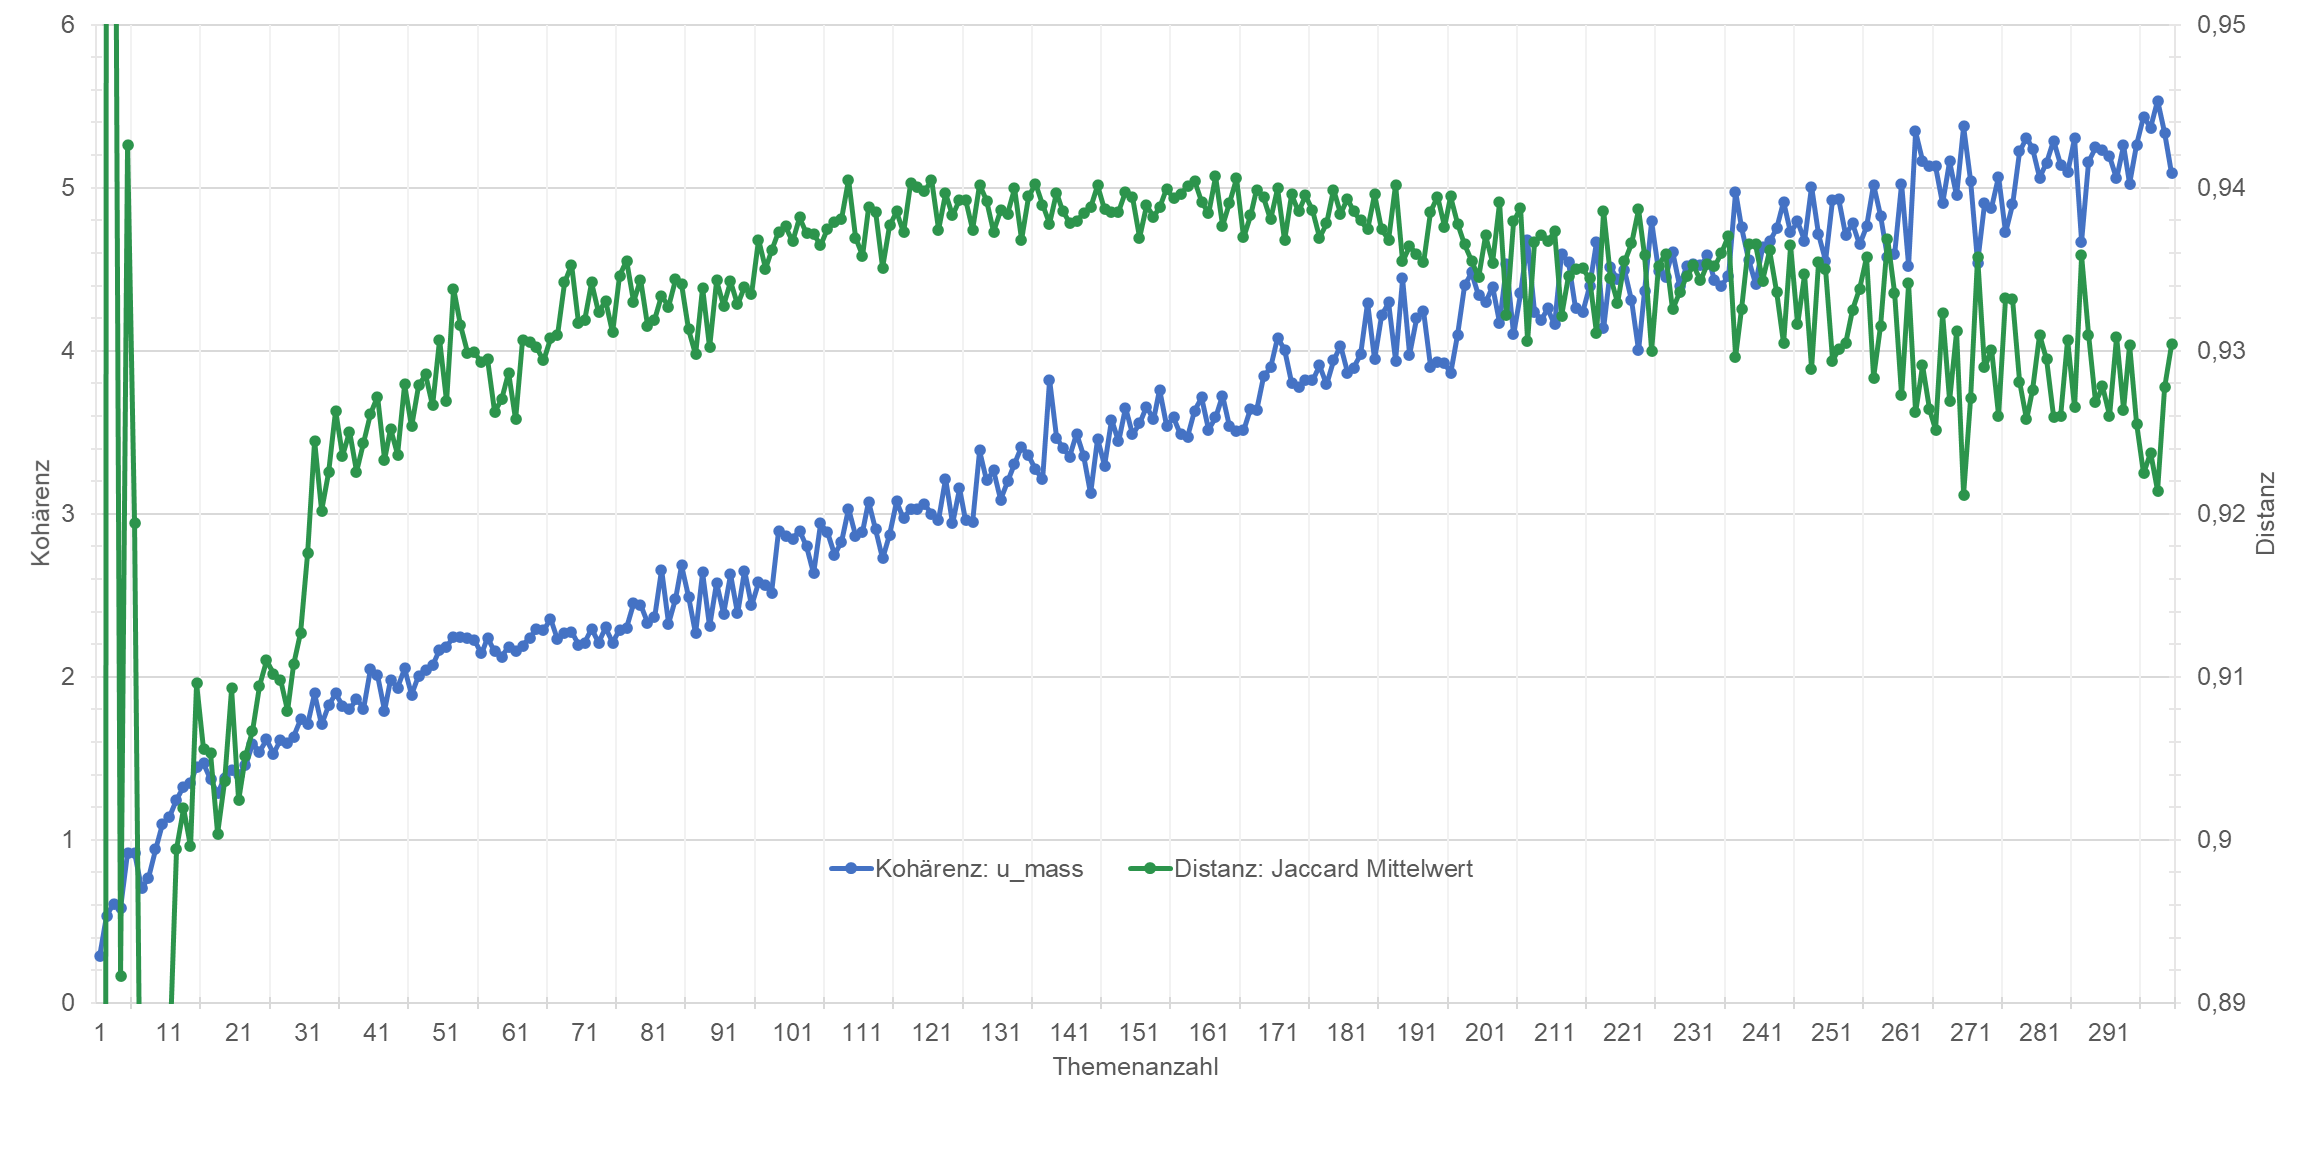
\includegraphics[width=\textwidth,keepaspectratio=true]{img/coherenceAndDistanceUnigram.png}
	\caption{
		Veränderung der Kohärenz- und Distanzwerte der Themen
	}
	\label{fig:Kohärenz_Distanz_Unigramme}
\end{figure}
\end{landscape}


Die Kohärenz der LDA Modelle wird mit dem u\_mass Maß bestimmt. Von eins wird der absolute u\_mass Wert vom LDA Modell mit n Themen subtrahiert und durch den absoluten u\_mass Wert des LDA Modells mit n + 1 Themen dividiert. Diese Berechnung wird für jedes Modell durchgeführt. Dadurch lässt sich die größte absolute Kohärenzsteigerung zum Vorgänger finden.

\begin{center}
	$1-\frac{\left|LDA n\right|}{\left|LDA n + 1\right|}$ 
\end{center}


Bei den Unigrammen sind es in Abbildung \ref{fig:Kohärenz_Distanz_Unigramme} 83 Themen. Bei den Bigrammen funktioniert diese Methode nicht so gut, um ein Plateau zu finden. Sie schlägt zehn Themen vor, was zu einem sehr groben Modell führt. Wie die Abbildung \ref{fig:Kohärenz_Distanz_Bigramme} zeigt wird eine hohe Kohärenz und Distanz bei der Themenanzahl von 51 erreicht. Mit der Anzahl wurde ein deutlich granulareres Modell erstellt. 

\begin{figure}[htpb]
	\centering
	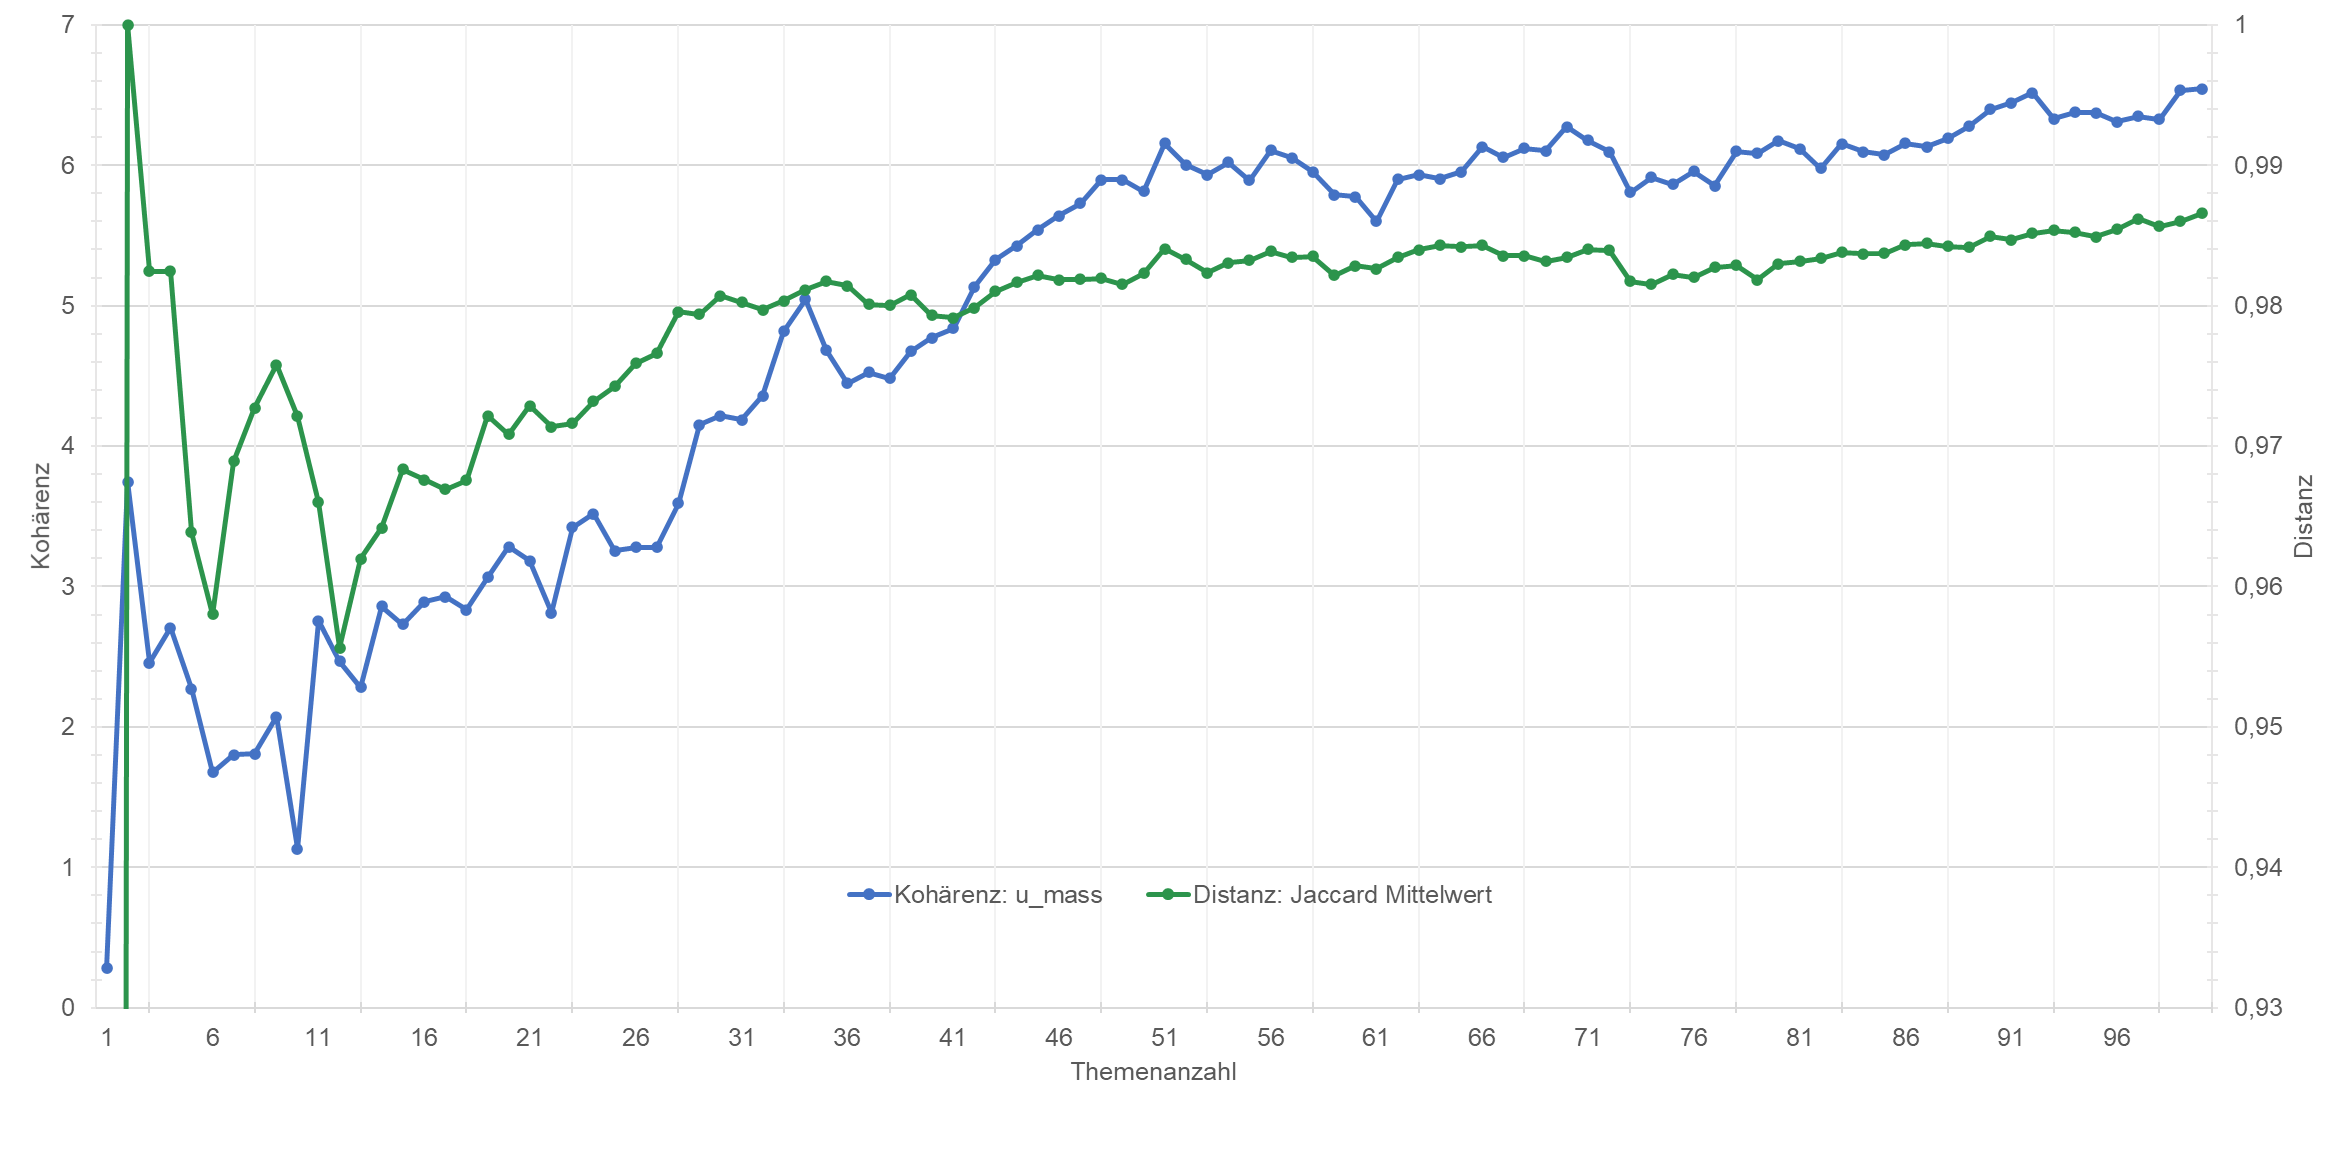
\includegraphics[width=\textwidth,height=10cm,keepaspectratio=true]{img/coherenceAndDistanceBigram.png}
	\caption{
		Kohärenz und Distanz der Themen mit Bigrammen
	}
	\label{fig:Kohärenz_Distanz_Bigramme}
\end{figure}


 

Im letzten Schritt werden die Daten als Themenliste, Dokument-Themen und Themen-Wort Matrizen gespeichert. Mit  pyLDAvis wird eine interaktive multidimensional skalierte Visualisierung erstellt. Diese Visualisierung berücksichtigt die Distanz und die Größe der Themen.


\subsection{Hierarchisches LDA}

Tomotopy ist ebenfalls eine Python library für Textanalyse. Sie ist ähnlich zu Gensim aber ist besonders performant und unterstützt zusätzlich \ac{hlda}, allerdings keine Kohärenzmaße. Deshalb werden hier beide librarys verwendet, um die jeweiligen Funktionen zu nutzen.

Die Wörter der Dokumente werden in eine Liste aus Listen geladen. Für \ac{hlda} wird keine Themenanzahl benötigt aber einige Parameter aus der Tabelle \ref{table:HLDA_Parameter} die \ac{lda} in Gensim selbst erlernt. Der \ac{hlda} verwirft die ersten 10.000 Iterationen und erstellt danach zehn Modelle mit einem Abstand von jeweils 100 Iterationen. \parencite[vgl.][S. 6]{griffiths2004hierarchical} \todo[inline]{25 random restarts to avoid local maxima, take highest posterior likelihood} In Abbildung \ref{fig:HLDA_Unigram_Baum} hat sich ein drei Ebenen tiefes Baumdiagramm als übersichtlich erwiesen, um Überthemen zu finden und Unterthemen zu clustern.

\begin{table}
	\RawFloats
	\centering
	\caption{HLDA Parameter}
	\begin{tabular}{|c|c|c|c|c|c|c|c|c|c|}
		\hline 
		Name& iter. & seed & TW & $\alpha$ & $\eta$ & $\gamma$ & depth & rm\_top & burn\_in \\ 
		\hline 
		Unigramme& 1000 & 100 & \ac{tf-idf} & 0,3 & 0,6 & 0,15 & 3 & 1 & 10.000 \\ 
		\hline 
		Bigramme& 1000 & 100 & \ac{tf-idf} & 0,3 & 0,6 & 0,15 & 3 & 1 & 10.000  \\ 
		\hline  
	\end{tabular}
	\label{table:HLDA_Parameter}
\end{table} 

Die Term Frequency-Inverse Document Frequency (\ac{tf-idf}) wird benutzt, um herauszufinden wie stark ein Wort zu einem Dokument gehört in einer Menge von Dokumenten. \parencite{luhn1957statistical}  \parencite{jones1972statistical} Der wert steigt mit mit der Frequenz des Wortes in einem Dokument und sinkt mit der Anzahl an Dokumenten in denen das Wort vorkommt.

\begin{figure}[htpb]
	\centering
	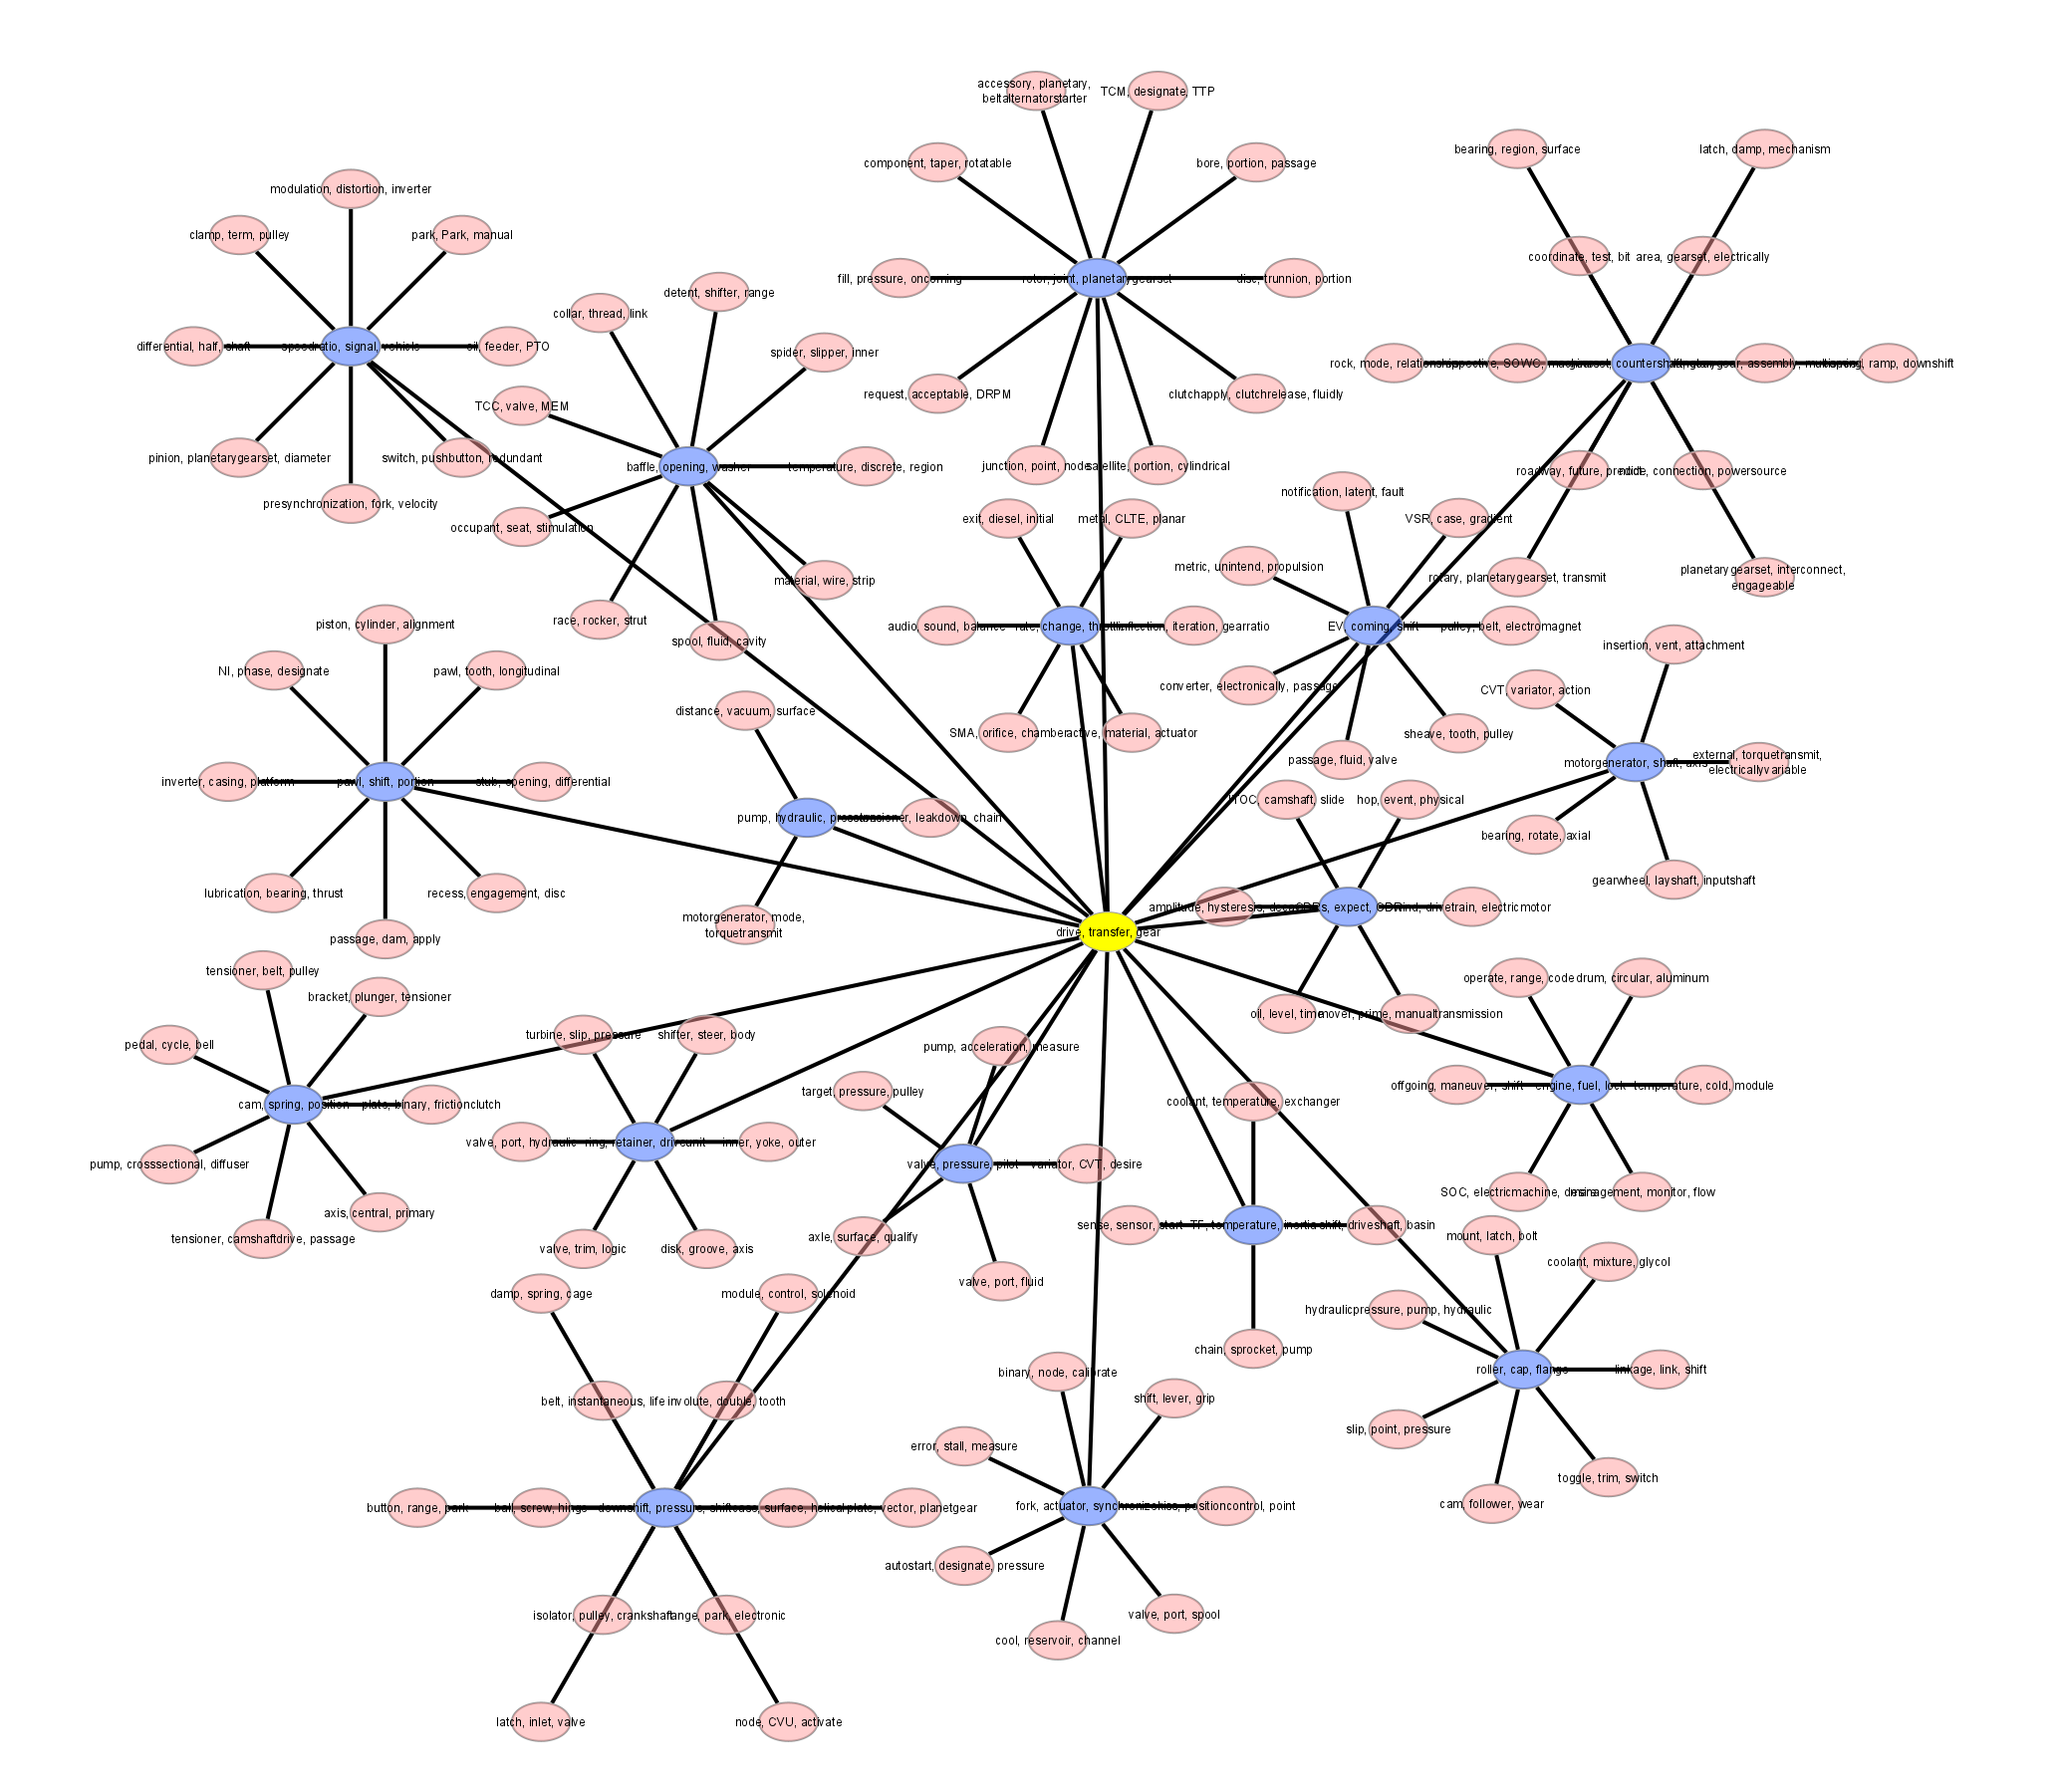
\includegraphics[height=15cm,width=\textwidth,keepaspectratio=true]{img/tree.png}
	\caption{
		HLDA Unigram Baumdiagramm
	}
	\label{fig:HLDA_Unigram_Baum}
\end{figure}

\subsection{Dynamisches LDA}

Für das \gls{dlda} wurden die 1410 Patente des Datensatzes in die 14 Zeitabschnitte von 2004 bis 2017 aufgeteilt. Jeder Zeitabschnitt ist ein Jahr lang und enthält die Patente deren APD in jenes Jahr fällt. Jeder Zeitabschnitt enthält 1 bis 173 Patente. Die Jahre 2004 und 2017 enthalten mit 1 und 13 Patenten die wenigsten im Datensatz. Damit die Ergebnisse des \gls{dlda} denen des \gls{lda} vergleichbar sind wurden für die Uni- und Bigramme wieder Modelle mit 83 und 51 Themen erstellt.

%\section{Gibbs Sampling}


